%===============================================================================
% LaTeX sjabloon voor de bachelorproef toegepaste informatica aan HOGENT
% Meer info op https://github.com/HoGentTIN/latex-hogent-report
%===============================================================================

\documentclass[dutch,dit,thesis]{hogentreport}

% TODO:
% - If necessary, replace the option `dit`' with your own department!
%   Valid entries are dbo, dbt, dgz, dit, dlo, dog, dsa, soa
% - If you write your thesis in English (remark: only possible after getting
%   explicit approval!), remove the option "dutch," or replace with "english".

\usepackage{lipsum} % For blind text, can be removed after adding actual content

%% Pictures to include in the text can be put in the graphics/ folder
\graphicspath{{../graphics/}}

%% For source code highlighting, requires pygments to be installed
%% Compile with the -shell-escape flag!
%% \usepackage[chapter]{minted}
%% If you compile with the make_thesis.{bat,sh} script, use the following
%% import instead:
\usepackage[chapter,outputdir=../output]{minted}
\usemintedstyle{solarized-light}

%% Formatting for minted environments.
\setminted{%
    autogobble,
    frame=lines,
    breaklines,
    linenos,
    tabsize=4
}

%% Ensure the list of listings is in the table of contents
\renewcommand\listoflistingscaption{%
    \IfLanguageName{dutch}{Lijst van codefragmenten}{List of listings}
}
\renewcommand\listingscaption{%
    \IfLanguageName{dutch}{Codefragment}{Listing}
}
\renewcommand*\listoflistings{%
    \cleardoublepage\phantomsection\addcontentsline{toc}{chapter}{\listoflistingscaption}%
    \listof{listing}{\listoflistingscaption}%
}

% Other packages not already included can be imported here

%%---------- Document metadata -------------------------------------------------
% TODO: Replace this with your own information
\author{Ernst Aarden}
\supervisor{Dhr. F. Van Houte}
\cosupervisor{Mevr. S. Beeckman}
\title[Optionele ondertitel]%
    {Titel van de bachelorproef}
\academicyear{\advance\year by -1 \the\year--\advance\year by 1 \the\year}
\examperiod{1}
\degreesought{\IfLanguageName{dutch}{Professionele bachelor in de toegepaste informatica}{Bachelor of applied computer science}}
\partialthesis{false} %% To display 'in partial fulfilment'
%\institution{Internshipcompany BVBA.}

%% Add global exceptions to the hyphenation here
\hyphenation{back-slash}

%% The bibliography (style and settings are  found in hogentthesis.cls)
\addbibresource{bachproef.bib}            %% Bibliography file
\addbibresource{../voorstel/voorstel.bib} %% Bibliography research proposal
\defbibheading{bibempty}{}

%% Prevent empty pages for right-handed chapter starts in twoside mode
\renewcommand{\cleardoublepage}{\clearpage}

\renewcommand{\arraystretch}{1.2}

%% Content starts here.
\begin{document}

%---------- Front matter -------------------------------------------------------

\frontmatter

\hypersetup{pageanchor=false} %% Disable page numbering references
%% Render a Dutch outer title page if the main language is English
\IfLanguageName{english}{%
    %% If necessary, information can be changed here
    \degreesought{Professionele Bachelor toegepaste informatica}%
    \begin{otherlanguage}{dutch}%
       \maketitle%
    \end{otherlanguage}%
}{}

%% Generates title page content
\maketitle
\hypersetup{pageanchor=true}

%%=============================================================================
%% Voorwoord
%%=============================================================================

\chapter*{\IfLanguageName{dutch}{Woord vooraf}{Preface}}%
\label{ch:voorwoord}

%% TODO:
%% Het voorwoord is het enige deel van de bachelorproef waar je vanuit je
%% eigen standpunt (``ik-vorm'') mag schrijven. Je kan hier bv. motiveren
%% waarom jij het onderwerp wil bespreken.
%% Vergeet ook niet te bedanken wie je geholpen/gesteund/... heeft

\lipsum[1-2]
%%=============================================================================
%% Samenvatting
%%=============================================================================

% TODO: De "abstract" of samenvatting is een kernachtige (~ 1 blz. voor een
% thesis) synthese van het document.
%
% Een goede abstract biedt een kernachtig antwoord op volgende vragen:
%
% 1. Waarover gaat de bachelorproef?
% 2. Waarom heb je er over geschreven?
% 3. Hoe heb je het onderzoek uitgevoerd?
% 4. Wat waren de resultaten? Wat blijkt uit je onderzoek?
% 5. Wat betekenen je resultaten? Wat is de relevantie voor het werkveld?
%
% Daarom bestaat een abstract uit volgende componenten:
%
% - inleiding + kaderen thema
% - probleemstelling
% - (centrale) onderzoeksvraag
% - onderzoeksdoelstelling
% - methodologie
% - resultaten (beperk tot de belangrijkste, relevant voor de onderzoeksvraag)
% - conclusies, aanbevelingen, beperkingen
%
% LET OP! Een samenvatting is GEEN voorwoord!

%%---------- Nederlandse samenvatting -----------------------------------------
%
% TODO: Als je je bachelorproef in het Engels schrijft, moet je eerst een
% Nederlandse samenvatting invoegen. Haal daarvoor onderstaande code uit
% commentaar.
% Wie zijn bachelorproef in het Nederlands schrijft, kan dit negeren, de inhoud
% wordt niet in het document ingevoegd.

\IfLanguageName{english}{%
\selectlanguage{dutch}
\chapter*{Samenvatting}
\lipsum[1-4]
\selectlanguage{english}
}{}

%%---------- Samenvatting -----------------------------------------------------
% De samenvatting in de hoofdtaal van het document

\chapter*{\IfLanguageName{dutch}{Samenvatting}{Abstract}}

\lipsum[1-4]


%---------- Inhoud, lijst figuren, ... -----------------------------------------

\tableofcontents

% In a list of figures, the complete caption will be included. To prevent this,
% ALWAYS add a short description in the caption!
%
%  \caption[short description]{elaborate description}
%
% If you do, only the short description will be used in the list of figures

\listoffigures

% If you included tables and/or source code listings, uncomment the appropriate
% lines.
\listoftables

\listoflistings

% Als je een lijst van afkortingen of termen wil toevoegen, dan hoort die
% hier thuis. Gebruik bijvoorbeeld de ``glossaries'' package.
% https://www.overleaf.com/learn/latex/Glossaries

%---------- Kern ---------------------------------------------------------------

\mainmatter{}

% De eerste hoofdstukken van een bachelorproef zijn meestal een inleiding op
% het onderwerp, literatuurstudie en verantwoording methodologie.
% Aarzel niet om een meer beschrijvende titel aan deze hoofdstukken te geven of
% om bijvoorbeeld de inleiding en/of stand van zaken over meerdere hoofdstukken
% te verspreiden!

%%=============================================================================
%% Inleiding
%%=============================================================================

\chapter{\IfLanguageName{dutch}{Inleiding}{Introduction}}%
\label{ch:inleiding}

De inleiding moet de lezer net genoeg informatie verschaffen om het onderwerp te begrijpen en in te zien waarom de onderzoeksvraag de moeite waard is om te onderzoeken. In de inleiding ga je literatuurverwijzingen beperken, zodat de tekst vlot leesbaar blijft. Je kan de inleiding verder onderverdelen in secties als dit de tekst verduidelijkt. Zaken die aan bod kunnen komen in de inleiding~\autocite{Pollefliet2011}:

\begin{itemize}
  \item context, achtergrond
  \item afbakenen van het onderwerp
  \item verantwoording van het onderwerp, methodologie
  \item probleemstelling
  \item onderzoeksdoelstelling
  \item onderzoeksvraag
  \item \ldots
\end{itemize}

\section{\IfLanguageName{dutch}{Probleemstelling}{Problem Statement}}%
\label{sec:probleemstelling}

Uit je probleemstelling moet duidelijk zijn dat je onderzoek een meerwaarde heeft voor een concrete doelgroep. De doelgroep moet goed gedefinieerd en afgelijnd zijn. Doelgroepen als ``bedrijven,'' ``KMO's'', systeembeheerders, enz.~zijn nog te vaag. Als je een lijstje kan maken van de personen/organisaties die een meerwaarde zullen vinden in deze bachelorproef (dit is eigenlijk je steekproefkader), dan is dat een indicatie dat de doelgroep goed gedefinieerd is. Dit kan een enkel bedrijf zijn of zelfs één persoon (je co-promotor/opdrachtgever).

\section{\IfLanguageName{dutch}{Onderzoeksvraag}{Research question}}%
\label{sec:onderzoeksvraag}

Wees zo concreet mogelijk bij het formuleren van je onderzoeksvraag. Een onderzoeksvraag is trouwens iets waar nog niemand op dit moment een antwoord heeft (voor zover je kan nagaan). Het opzoeken van bestaande informatie (bv. ``welke tools bestaan er voor deze toepassing?'') is dus geen onderzoeksvraag. Je kan de onderzoeksvraag verder specifiëren in deelvragen. Bv.~als je onderzoek gaat over performantiemetingen, dan 

\section{\IfLanguageName{dutch}{Onderzoeksdoelstelling}{Research objective}}%
\label{sec:onderzoeksdoelstelling}

Wat is het beoogde resultaat van je bachelorproef? Wat zijn de criteria voor succes? Beschrijf die zo concreet mogelijk. Gaat het bv.\ om een proof-of-concept, een prototype, een verslag met aanbevelingen, een vergelijkende studie, enz.

\section{\IfLanguageName{dutch}{Opzet van deze bachelorproef}{Structure of this bachelor thesis}}%
\label{sec:opzet-bachelorproef}

% Het is gebruikelijk aan het einde van de inleiding een overzicht te
% geven van de opbouw van de rest van de tekst. Deze sectie bevat al een aanzet
% die je kan aanvullen/aanpassen in functie van je eigen tekst.

De rest van deze bachelorproef is als volgt opgebouwd:

In Hoofdstuk~\ref{ch:stand-van-zaken} wordt een overzicht gegeven van de stand van zaken binnen het onderzoeksdomein, op basis van een literatuurstudie.

In Hoofdstuk~\ref{ch:methodologie} wordt de methodologie toegelicht en worden de gebruikte onderzoekstechnieken besproken om een antwoord te kunnen formuleren op de onderzoeksvragen.

% TODO: Vul hier aan voor je eigen hoofstukken, één of twee zinnen per hoofdstuk

In Hoofdstuk~\ref{ch:conclusie}, tenslotte, wordt de conclusie gegeven en een antwoord geformuleerd op de onderzoeksvragen. Daarbij wordt ook een aanzet gegeven voor toekomstig onderzoek binnen dit domein.
\chapter{\IfLanguageName{dutch}{Stand van zaken}{State of the art}}%
\label{ch:stand-van-zaken}

% Tip: Begin elk hoofdstuk met een paragraaf inleiding die beschrijft hoe
% dit hoofdstuk past binnen het geheel van de bachelorproef. Geef in het
% bijzonder aan wat de link is met het vorige en volgende hoofdstuk.

% Pas na deze inleidende paragraaf komt de eerste sectiehoofding.

Dit hoofdstuk bevat je literatuurstudie. De inhoud gaat verder op de inleiding, maar zal het onderwerp van de bachelorproef *diepgaand* uitspitten. De bedoeling is dat de lezer na lezing van dit hoofdstuk helemaal op de hoogte is van de huidige stand van zaken (state-of-the-art) in het onderzoeksdomein. Iemand die niet vertrouwd is met het onderwerp, weet nu voldoende om de rest van het verhaal te kunnen volgen, zonder dat die er nog andere informatie moet over opzoeken \autocite{Pollefliet2011}.

Je verwijst bij elke bewering die je doet, vakterm die je introduceert, enz.\ naar je bronnen. In \LaTeX{} kan dat met het commando \texttt{$\backslash${textcite\{\}}} of \texttt{$\backslash${autocite\{\}}}. Als argument van het commando geef je de ``sleutel'' van een ``record'' in een bibliografische databank in het Bib\LaTeX{}-formaat (een tekstbestand). Als je expliciet naar de auteur verwijst in de zin (narratieve referentie), gebruik je \texttt{$\backslash${}textcite\{\}}. Soms is de auteursnaam niet expliciet een onderdeel van de zin, dan gebruik je \texttt{$\backslash${}autocite\{\}} (referentie tussen haakjes). Dit gebruik je bv.~bij een citaat, of om in het bijschrift van een overgenomen afbeelding, broncode, tabel, enz. te verwijzen naar de bron. In de volgende paragraaf een voorbeeld van elk.

\textcite{Knuth1998} schreef een van de standaardwerken over sorteer- en zoekalgoritmen. Experten zijn het erover eens dat cloud computing een interessante opportuniteit vormen, zowel voor gebruikers als voor dienstverleners op vlak van informatietechnologie~\autocite{Creeger2009}.

Let er ook op: het \texttt{cite}-commando voor de punt, dus binnen de zin. Je verwijst meteen naar een bron in de eerste zin die erop gebaseerd is, dus niet pas op het einde van een paragraaf.

\begin{figure}
  \centering
  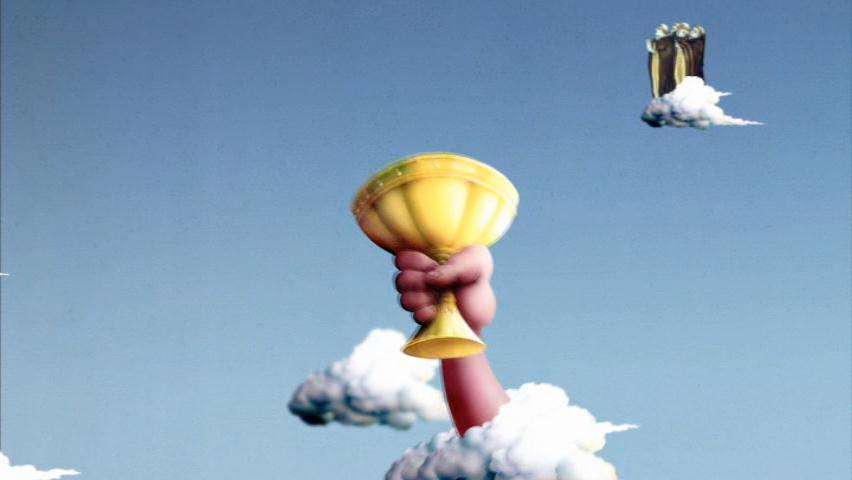
\includegraphics[width=0.8\textwidth]{grail.jpg}
  \caption[Voorbeeld figuur.]{\label{fig:grail}Voorbeeld van invoegen van een figuur. Zorg altijd voor een uitgebreid bijschrift dat de figuur volledig beschrijft zonder in de tekst te moeten gaan zoeken. Vergeet ook je bronvermelding niet!}
\end{figure}

\begin{listing}
  \begin{minted}{python}
    import pandas as pd
    import seaborn as sns

    penguins = sns.load_dataset('penguins')
    sns.relplot(data=penguins, x="flipper_length_mm", y="bill_length_mm", hue="species")
  \end{minted}
  \caption[Voorbeeld codefragment]{Voorbeeld van het invoegen van een codefragment.}
\end{listing}

\lipsum[7-20]

\begin{table}
  \centering
  \begin{tabular}{lcr}
    \toprule
    \textbf{Kolom 1} & \textbf{Kolom 2} & \textbf{Kolom 3} \\
    $\alpha$         & $\beta$          & $\gamma$         \\
    \midrule
    A                & 10.230           & a                \\
    B                & 45.678           & b                \\
    C                & 99.987           & c                \\
    \bottomrule
  \end{tabular}
  \caption[Voorbeeld tabel]{\label{tab:example}Voorbeeld van een tabel.}
\end{table}


%%=============================================================================
%% Methodologie
%%=============================================================================

\chapter{\IfLanguageName{dutch}{Methodologie}{Methodology}}%
\label{ch:methodologie}

%% TODO: In dit hoofstuk geef je een korte toelichting over hoe je te werk bent
%% gegaan. Verdeel je onderzoek in grote fasen, en licht in elke fase toe wat
%% de doelstelling was, welke deliverables daar uit gekomen zijn, en welke
%% onderzoeksmethoden je daarbij toegepast hebt. Verantwoord waarom je
%% op deze manier te werk gegaan bent.
%% 
%% Voorbeelden van zulke fasen zijn: literatuurstudie, opstellen van een
%% requirements-analyse, opstellen long-list (bij vergelijkende studie),
%% selectie van geschikte tools (bij vergelijkende studie, "short-list"),
%% opzetten testopstelling/PoC, uitvoeren testen en verzamelen
%% van resultaten, analyse van resultaten, ...
%%
%% !!!!! LET OP !!!!!
%%
%% Het is uitdrukkelijk NIET de bedoeling dat je het grootste deel van de corpus
%% van je bachelorproef in dit hoofstuk verwerkt! Dit hoofdstuk is eerder een
%% kort overzicht van je plan van aanpak.
%%
%% Maak voor elke fase (behalve het literatuuronderzoek) een NIEUW HOOFDSTUK aan
%% en geef het een gepaste titel.

\lipsum[21-25]



% Voeg hier je eigen hoofdstukken toe die de ``corpus'' van je bachelorproef
% vormen. De structuur en titels hangen af van je eigen onderzoek. Je kan bv.
% elke fase in je onderzoek in een apart hoofdstuk bespreken.

%\input{...}
%\input{...}
%...

%%=============================================================================
%% Conclusie
%%=============================================================================

\chapter{Conclusie}%
\label{ch:conclusie}

% TODO: Trek een duidelijke conclusie, in de vorm van een antwoord op de
% onderzoeksvra(a)g(en). Wat was jouw bijdrage aan het onderzoeksdomein en
% hoe biedt dit meerwaarde aan het vakgebied/doelgroep? 
% Reflecteer kritisch over het resultaat. In Engelse teksten wordt deze sectie
% ``Discussion'' genoemd. Had je deze uitkomst verwacht? Zijn er zaken die nog
% niet duidelijk zijn?
% Heeft het onderzoek geleid tot nieuwe vragen die uitnodigen tot verder 
%onderzoek?

\lipsum[76-80]



%---------- Bijlagen -----------------------------------------------------------

\appendix

\chapter{Onderzoeksvoorstel}

Het onderwerp van deze bachelorproef is gebaseerd op een onderzoeksvoorstel dat vooraf werd beoordeeld door de promotor. Dat voorstel is opgenomen in deze bijlage.

%% TODO: 
%\section*{Samenvatting}

% Kopieer en plak hier de samenvatting (abstract) van je onderzoeksvoorstel.

% Verwijzing naar het bestand met de inhoud van het onderzoeksvoorstel
%---------- Inleiding ---------------------------------------------------------

% TODO: Is dit voorstel gebaseerd op een paper van Research Methods die je
% vorig jaar hebt ingediend? Heb je daarbij eventueel samengewerkt met een
% andere student?
% Zo ja, haal dan de tekst hieronder uit commentaar en pas aan.

%\paragraph{Opmerking}

% Dit voorstel is gebaseerd op het onderzoeksvoorstel dat werd geschreven in het
% kader van het vak Research Methods dat ik (vorig/dit) academiejaar heb
% uitgewerkt (met medesturent VOORNAAM NAAM als mede-auteur).
% 

\section{Inleiding}%
\label{sec:inleiding}

In de hedendaagse digitale wereld evolueert de manier waarop advertenties worden geïtegreerd in videostreamingplatforms sneller dan ooit. Recente ontwikkelingen bij YouTube suggereren een verandering naar server-side ad injection, waar adverenties direct in de videostream worden geïntegreergd \cite{Li2024}. Deze technische verandering maakt de tranditionele methodes van advertentiedetectie en -blokkering, zoals adblockers, minder effectief.

Dit onderzoek focust zich op de technische haalbaarheid van het detecteren van geïntegreerde advertenties in MP4-videobestanden met behulp van computer vision technieken in real-time. De primaire doelgroep zijn softwareontwikkelaars die software ontwikkelen voor contentanalyse. Het onderzoek focust specifiek op oplossingen die lokaal kunnen draaien op standaard consumentenlaptops, zonder afhankelijk te zijn van cloudservices, of grote rekenkracht.

De centrale onderzoeksvraag is: \textit{"Is het mogelijk om met behulp van computer vision een lichtgewicht oplossing te ontwikkelen die advertenties in MP4-bestanden kan detecteren met een accuraatheid van 90\%, gebruikmakend van alleen lokale rekenkracht?"} Bestaande onderzoeken, zoals dat van \textcite{Covell2007}, hebben aangetoond dat advertentiedetectie mogelijk is door gebruik te maken van zowel audio- als visuele kenmerken, maar vereisen vaak substantiële verwerkingskracht en zijn niet ontworpen voor individueel gebruik.

Het doel van dit onderzoek is het ontwikkelen van een proof-of-concept dat:
\begin{itemize}
   \item Advertenties kan detecteren binnen één seconde na het afspelen
   \item Een accuraatheid van minimaal 90\% behaalt
   \item Effectief werkt op diverse soorten video-inhoud en advertenties
   \item Draait op standaard consumentenhardware
\end{itemize}

De relevantie van dit onderzoek wordt onderstreept door de voortdurende technische evolutie van reclamedistributie in online video's, en de behoefte aan toegankelijke tools voor contentanalyse. Het eindresultaat zal bestaan uit een werkende proof-of-concept implementatie en een analyse van de haalbaarheid van lokale advertentiedetectie, inclusief prestatiemetingen en suggesties voor verdere ontwikkeling.

%---------- Stand van zaken ---------------------------------------------------

\section{Literatuurstudie}%
\label{sec:literatuurstudie}

\subsection{Evolutie van Video Advertenties}
De manier waarop advertenties worden geïntegreerd in videoplatforms is significant geëvolueerd. Waar advertenties oorspronkelijk werden geladen via aparte client-side requests, verschuift de trend nu naar server-side ad injection \autocite{Li2024}. YouTube experimenteert momenteel met het direct embedden van advertenties in de videostream, wat traditionele advertentiedetectie methodes ineffectief maakt.

\subsection{Bestaande Detectie Methodes}
Verschillende onderzoekers hebben methodes ontwikkeld voor het detecteren van advertenties in videostreams. \textcite{Covell2007} presenteerden een aanpak die zowel audio- als visuele kenmerken gebruikt om herhaalde advertenties te identificeren. Deze methode behaalde een precisie van meer dan 99\% en een recall van 95\%, maar vereist substantiële verwerkingskracht en is niet ontworpen voor real-time verwerking op consumentenhardware.

\subsection{Machine Learning Benaderingen}
Recente ontwikkelingen in machine learning hebben nieuwe mogelijkheden geopend voor videoclassificatie. \textcite{Liu2023} demonstreerden een deep learning framework dat individuele advertenties kan detecteren en segmenteren met behulp van een combinatie van audio- en visuele analyse. Hun aanpak gebruikt een lichtgewicht audio-gebaseerde segmentatie gevolgd door een diepere visuele analyse, wat efficiënter is dan pure videogebaseerde methodes.

\subsection{Technische Uitdagingen}
Het ontwikkelen van een effectieve advertentiedetectie oplossing voor consumentenhardware brengt verschillende uitdagingen met zich mee:

\begin{itemize}
    \item \textbf{Verwerkingskracht}: Consumer hardware heeft vaak beperkte GPU-capaciteit voor real-time videoverwerking.
    \item \textbf{Real-time Prestaties}: Deep learning modellen zijn computationeel intensief, wat real-time detectie moeilijker maakt zonder high-end hardware.
    \item \textbf{Nauwkeurigheid vs. Efficiëntie}: Lichtgewicht modellen zijn sneller maar kunnen minder nauwkeurig zijn in advertentiedetectie.
\end{itemize}

\subsection{Aanwezige Uitdagingen}
Uit de literatuur blijkt dat er nog verschillende open vraagstukken zijn:

\begin{itemize}
    \item Het ontwikkelen van efficiënte detectiemethodes die lokaal kunnen draaien op consumentenhardware
    \item Het bereiken van real-time prestaties zonder toegeving te doen aan de accuraatheid
    \item Het omgaan met geïntegreerde advertenties die steeds meer op reguliere content lijken
\end{itemize}

%---------- Methodologie ------------------------------------------------------
\section{Methodologie}%
\label{sec:methodologie}

Dit onderzoek volgt een systematische aanpak voor het ontwikkelen en evalueren van een lichtgewicht advertentiedetectiesysteem. De methodologie is opgedeeld in vijf hoofdfasen.

\subsection{Technologisch Onderzoek (4 weken)}
\begin{itemize}
    \item Literatuurstudie naar bestaande oplossingen
    \item Evaluatie van potentiële technologieën:
    \begin{itemize}
        \item Computer Vision: OpenCV
        \item Machine Learning: PyTorch, TensorFlow, Scikit-learn
        \item Video Processing: FFmpeg, OpenCV
        \item Data Analyse: NumPy, Pandas, Seaborn
    \end{itemize}
    \item Analyse van hardware vereisten op consumentenhardware
\end{itemize}

\subsection{Data Verzameling (4 weken)}
\begin{itemize}
    \item Ontwikkelen van een systematische verzamelingstrategie:
    \begin{itemize}
        \item Matrix van variabelen voor diverse videocontent
        \item 10 videos per unieke combinatie van eigenschappen
    \end{itemize}
    \item Ontwikkeling van dataverwerkingsscripts:
    \begin{itemize}
        \item Video normalisatie (720p resolutie)
        \item Advertentie injectie tool
        \item Generatie van gepaarde JSON bestanden met tijdsmarkeringen
    \end{itemize}
    \item Verzamelen van 100-200 testvideos en advertenties
\end{itemize}

\subsection{Ontwikkeling (8 weken)}
\begin{itemize}
    \item Implementatie van kernfunctionaliteiten:
    \begin{itemize}
        \item Segmentatie van video in 1-minuut analyseerbare delen
        \item Buffer systeem voor vooruitlopende analyse
        \item Detectie algoritme met CPU-focus
        \item Optionele GPU-acceleratie via CUDA indien nodig
    \end{itemize}
    \item Containerisatie met Docker voor consistente uitvoering
    \item Ontwikkeling van performantiemonitoringsysteem
\end{itemize}

\subsection{Testen en Analyse (4 weken)}
\begin{itemize}
    \item Performantietests:
    \begin{itemize}
        \item CPU gebruik meting via Python's psutil library
        \item Geheugengebruik monitoring
        \item Frame-by-frame verwerkingstijd analyse
        \item End-to-end systeemlatentie metingen
    \end{itemize}
    \item Accuraatheidsmetingen:
    \begin{itemize}
        \item Precision en recall per advertentietype
        \item False positive/negative analyse
        \item Analyse van detectiefouten per contenttype
    \end{itemize}
    \item Cross-platform tests op verschillende hardware configuraties
\end{itemize}

\subsection{Documentatie en Afronding (4 weken)}
\begin{itemize}
    \item Schrijven van technische documentatie
    \item Analyse van resultaten en formuleren van conclusies
    \item Voorbereiden van presentatie en demonstratie
    \item GitHub repository documentatie en installatie-instructies
\end{itemize}

\subsection{Ontwikkelomgeving en Tools}
\begin{itemize}
    \item Ontwikkelomgeving: VSCode met Python plugins
    \item Versiebeheer: Git/GitHub
    \item Containerisatie: Docker voor reproduceerbare omgeving
    \item Programmeertaal: Python 3.x
    \item Hardware: Tests op verschillende consumentenlaptops
\end{itemize}

%---------- Verwachte resultaten ----------------------------------------------
\section{Verwacht resultaat, conclusie}%
\label{sec:verwachte_resultaten}

\subsection{Verwachte Meetresultaten}

We verwachten de volgende meetbare resultaten te kunnen demonstreren:

\begin{itemize}
    \item \textbf{CPU Gebruik}:
    \begin{itemize}
        \item Gemiddeld gebruik rond 60\%
        \item Piekgebruik niet hoger dan 80\%
        \item Stabiel gebruikspatroon zonder onverwachte pieken
    \end{itemize}
    
    \item \textbf{Detectie Accuraatheid}:
    \begin{itemize}
        \item Gemiddelde accuraatheid van 90\%
        \item Minimale accuraatheid niet lager dan 85\%
        \item Hogere accuraatheid voor kortere advertenties
        \item Verwachte uitdagingen bij extreem lange advertenties (>10 minuten)
    \end{itemize}
    
    \item \textbf{Reactietijd}:
    \begin{itemize}
        \item Detectie binnen 1 seconde na start advertentie
        \item Consistente prestaties ongeacht video lengte
    \end{itemize}
\end{itemize}

\subsection{Verwachte Visualisaties}
Om de resultaten inzichtelijk te maken, zullen de volgende grafieken worden gegenereerd:

\begin{itemize}
    \item CPU gebruiksgrafiek over tijd
    \item Accuraatheid per advertentietype
    \item Reactietijd analyse
    \item Geheugengebruik patroon
    \item Detectie accuraatheid vs. advertentie lengte
    \item Analyse van false positives per content type
\end{itemize}

\subsection{Meerwaarde voor Doelgroep}
Dit onderzoek zal op verschillende manieren bijdragen aan het vakgebied:

\begin{itemize}
    \item \textbf{Voor Ontwikkelaars}:
    \begin{itemize}
        \item Inzicht in real-time video analyse technieken
        \item Identificatie van veelvoorkomende bottlenecks en oplossingen
        \item Open-source implementatie voor verder onderzoek
    \end{itemize}
    
    \item \textbf{Voor het Vakgebied}:
    \begin{itemize}
        \item Nieuwe inzichten in lokale video processing
        \item Benchmark voor prestaties op consumentenhardware
        \item Basis voor toekomstige optimalisaties
    \end{itemize}
\end{itemize}

\subsection{Verwachte Uitdagingen en Beperkingen}
We anticiperen de volgende uitdagingen:

\begin{itemize}
    \item Hardware limitaties op consumentenapparatuur
    \item Verminderde accuraatheid bij extreme advertentielengtes
    \item Moeilijkheden bij het onderscheiden van user-generated advertenties
    \item Trade-offs tussen snelheid en accuraatheid
    \item Beperking tot MP4-videobestanden als inputformaat
\end{itemize}

\subsection{Onderzoekshypotheses}
Onze hoofdhypotheses zijn:

\begin{itemize}
    \item Lokale verwerking is haalbaar met acceptabele compromissen in accuraatheid
    \item Computer vision alleen zal ongeveer 50\% accuraatheid bereiken
    \item Machine learning technieken kunnen de accuraatheid significant verbeteren
    \item Een lichtgewicht model kan real-time presteren op consumentenhardware
\end{itemize}

Mocht uit het onderzoek blijken dat deze hypotheses niet kloppen, dan zal dit waardevolle inzichten opleveren over de werkelijke uitdagingen van lokale video-analyse en mogelijke alternatieve benaderingen, zoals hybride oplossingen met cloud computing.



%%---------- Andere bijlagen --------------------------------------------------
% TODO: Voeg hier eventuele andere bijlagen toe. Bv. als je deze BP voor de
% tweede keer indient, een overzicht van de verbeteringen t.o.v. het origineel.
%\input{...}

%%---------- Backmatter, referentielijst ---------------------------------------

\backmatter{}

\setlength\bibitemsep{2pt} %% Add Some space between the bibliograpy entries
\printbibliography[heading=bibintoc]

\end{document}
